\documentclass[a4paper,12pt]{article} 

\usepackage[unicode, pdftex]{hyperref}

%Добавляет возможность искать и копировать текст
\usepackage{cmap}

%Убирает пробел между названием таблицы/рисунка и самой таблицей/рисунком
\usepackage{caption}
\captionsetup[table]{skip= -0 cm}
\captionsetup[figure]{skip= -0 cm}

%Выравнивание названия таблиц по левому краю
%\usepackage[nooneline]{caption} 
%Размеры отступов 
\usepackage[left=20mm, top=20mm, right=20mm, bottom=20mm, footskip=10mm]{geometry}

%Рисунки
\usepackage{graphicx}
\usepackage{wrapfig} %обтекание элементов
\graphicspath{{graphs}{figures}}  % папки с картинками

%Русский язык в формулах
\usepackage{mathtext}

%  Русский язык
\usepackage[T2A]{fontenc}			
\usepackage[utf8]{inputenc}			
\usepackage[english,russian]{babel}	

%Красная строка для первого абзаца
\usepackage{indentfirst}

%Готические буквы
\usepackage{amssymb}

% Математика
\usepackage{amsmath,amsfonts,amssymb,amsthm,mathtools} 
\usepackage{wasysym}

%Цветные подписи в таблице
\usepackage[table,xcdraw]{xcolor}

\usepackage{fancyhdr} % Колонтитулы
 	\pagestyle{fancy}
 	\renewcommand{\headrulewidth}{0.3mm}  % Толщина линейки, отчеркивающей верхний колонтитул
 	%\lfoot{Нижний левый}
 	%\rfoot{Нижний правый}
 	\rhead{Белостоцкий Артмемий, Б04-006}
 	%\chead{Верхний в центре}
 	\lhead{Лабораторная работа №11.1}
 	\renewcommand{\footrulewidth}{0.3mm}
 	\cfoot{\thepage} % По умолчанию здесь номер страницы
 	
 	
%\captionsetup[table]{
%  position=above,
%  justification=raggedright,
  %labelsep=newline, % <<< label and text on different lines
%  singlelinecheck=false % <<< raggadright also when the cap%tion is shorter
                        % than a single line
%}
 	
\begin{document} 

%Титульник 
\begin{titlepage}
	\begin{center}
		\large 	МИНИСТЕРСТВО ОБРАЗОВАНИЯ И НАУКИ РОССИЙСКОЙ ФЕДЕРАЦИИ\\
				МОСКОВСКИЙ ФИЗИКО-ТЕХНИЧЕСКИЙ ИНСТИТУТ \\
				(НАЦИОНАЛЬНЫЙ ИССЛЕДОВАТЕЛЬСКИЙ ИНСТИТУТ)\\ 
				ФИЗТЕХ-ШКОЛА ЭЛЕКТРОНИКИ, ФОТОНИКИ \\
				И МОЛЕКУЛЯРНОЙ ФИЗИКИ \\
		
		
		\vspace{4.0 cm}
		Лабораторная работа № 11.1 \\
		\LARGE \textbf{Определение ширины запрещенной зоны полупроводника.}
	\end{center}
	\vspace{3 cm} \large
	
	\begin{flushright}
		выполнил студент 3 курса \\
		{группы Б04-006}\\
		\textbf{Белостоцкий Артемий}\\
	\end{flushright}
	
	\vfill

	\begin{center}
	Долгопрудный, 2023 г.
	\end{center}
\end{titlepage}                                                                      

\section*{Аннотация}

В данной работе исследуется температурная зависимость проводимости полупроводников -- германия и кремния, а также определяется ширина запрещенной зоны.

\section*{Теоретические сведения}

\subsection*{Разрешенные и запрещенные зоны в твердых телах}

В твердых телах атомы близко подходят друг к другу и не могут взаимодействовать как независимые. Задача о положении уровней взаимодействующих атомов очень сложна и не может быть исследована простыми методами. Основные эффекты, которые возникают при таком взаимодействии, близки к эффектам происходящим при взаимодействии классических колебательных систем -- две одинаковые системы с равными собственными частотами при взаимодействии характеризуются двумя коллективными колебаниями со слегка <<расщепившимися>> частотами \footnote{Доказательство данного факта можно найти в \cite{goldin}}. 

В квантовой механике подобное <<расщепление>> частот происходит в кристаллах, состоящих из большого числа взаимодействующих между собой атомов.Наиболее сильно выражено расщепление <<верхних>>  уровней, связанное с тем, что внешние электроны слабее всего связаны со своими атомами и могут <<подходить>> к другим атомам. Уровни, образовавшиеся при расщеплении каждого атомного уровня, образуют \textit{разрешенную зону}. Разрешенные зоны разделены между собой свободными от уровней энергетическими промежутками, которые называют \textit{запрещенными зонами}.

\begin{figure}[h!]
	\centering
	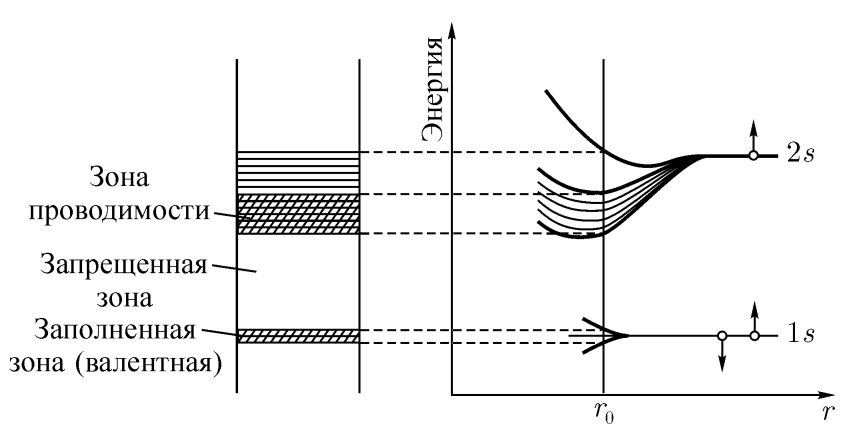
\includegraphics[width=\linewidth]{zones_in_solids}
	\caption{Образование разрешенных зон из одиночных уровней. Взято из \cite{goldin}}
\end{figure}

Следует подчеркнуть, что образование зон из атомных уровней происходит во всех кристаллах, независимо от их типа. Различие между кристаллами состоит не в наличии или отсутствии зон, а в расположении зон и в характере их заполнения.

\pagebreak

\subsection*{Некоторые сведения о полупроводниках}

\textit{Полупроводниками} называются кристаллы, которые при комнатной температуре проводят электрический ток, а при низких температурах являются изоляторами.

Величина электропроводности в полупроводниках определяется числом электронов в зоне проводимости, оно в свою очередь равно произведению числа имеющихся уровней на вероятность их заполнения. Вероятность заполнения уровней определятся функцией Ферми, которая при не очень высоких температурах имеет вид:

\begin{align}
	f(E) = \frac{1}{\exp \left( \frac{E - \mu }{kT}\right) - 1} \approx \exp \left( \frac{E - \mu }{kT}\right),
\end{align}

где E -- энергия уровня в зоне проводимости, $\mu$ -- некоторая константа, называемая энергией Ферми.

\begin{figure}[h!]
	\centering
	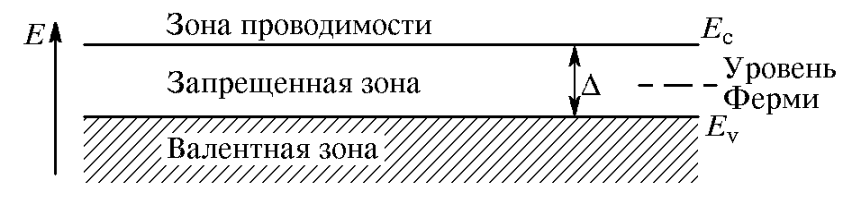
\includegraphics[width=0.8\linewidth]{semiconductor}
	\caption{Схема энергетических зон в полупроводнике. Взято из \cite{lab}}
\end{figure}

Число электронов в зоне проводимости определяется выражением:

\begin{align}
	n_n = Q_n \exp \left( - \frac{E_c - \mu}{kT} \right),
\end{align}

где $Q_n$ -- некоторое эффективное число уровней, находящихся вблизи дна зоны.

Вероятность появления дырки в валентной зоне определяется разностью $1 - f(E)$, поэтому число дырок равно:

\begin{align}
	n_p \approx Q_p \exp \left( - \frac{E_v - \mu}{kT} \right)
\end{align}

Учитывая, что мы рассматриваем чистый полупроводник (без примесей) получим, что $n_p = n_n =n$, тогда получим:

\begin{align} \label{eq4:number_of_electrons}
	n = C \exp \left( - \frac{\Delta}{2kT} \right)
\end{align}

Для нахождения электропроводности проводника вводят понятие подвижности электронов и дырок в электрическом поле -- $\mu_n$ и $\mu_p$ соответственно. По определению, средняя скорость электронов в электрическом поле $v_{ср} = \mu \varepsilon$, где $\varepsilon$ -- напряженность электрического поля.

Вспоминая закон Ома в дифференциальной форме ($j = \sigma \varepsilon$) и выражение для плотности тока ($j = n |e| v_{ср}$), а также учитывая (\ref{eq4:number_of_electrons}), получим:

\begin{align} \label{eq5:dependence_of_temperature}
	\sigma = |e| C (\mu_n + \mu_p) \exp \left( - \frac{\Delta}{2kT} \right) = A \exp \left( - \frac{\Delta}{2kT} \right)
\end{align}

\pagebreak

\section*{Экспериментальная установка}

\begin{figure}[h!]
	\centering
	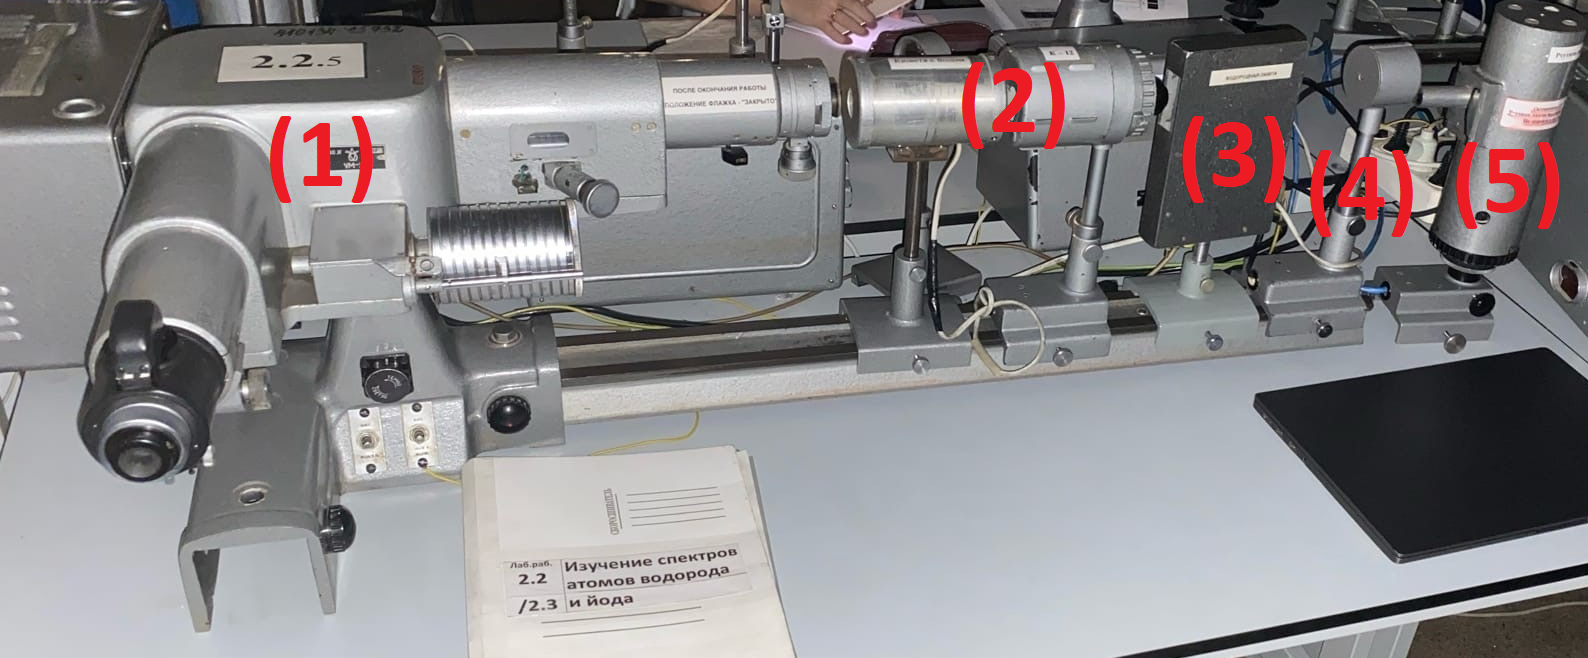
\includegraphics[width=0.8\linewidth]{setup}
	\caption{Экспериментальная установка. (1) -- электронагревательная печь, (2) -- магазин сопротивлений, (3) -- звуковой генератор, (4) -- вольтметр, снимающих показания термопары, (5) -- осциллограф, подключенных к мосту сопротивлений}
	\label{fig3:setup}
\end{figure}

\begin{figure}[h!]
	\centering
	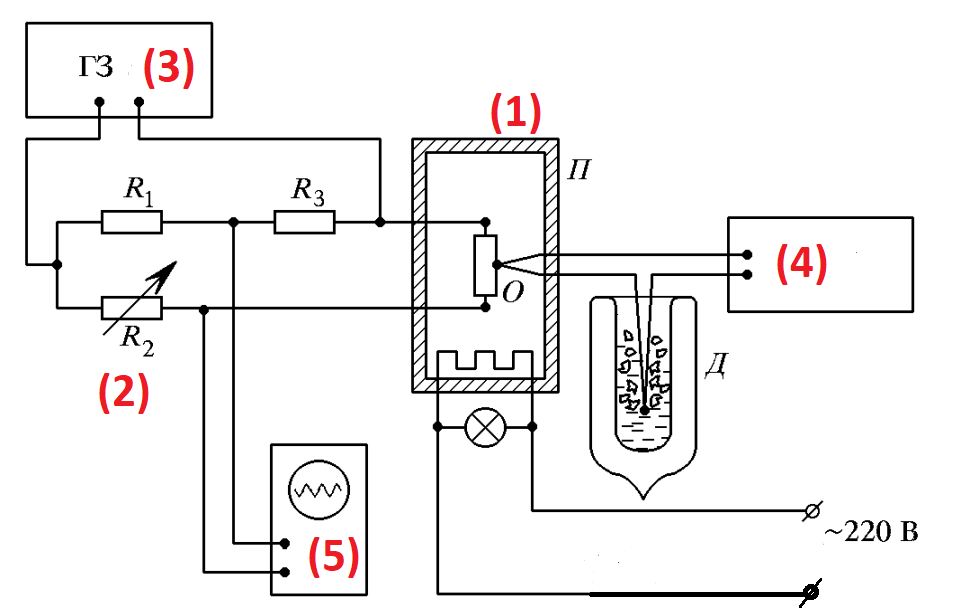
\includegraphics[width=0.8\linewidth]{scheme}
	\caption{Схема экспериментальной усатновки. O -- образец полупроводника, Д -- сосуд Дьюара, находящийся при комнатной температуре, остальные обозначения взяты из Рис.\ref{fig3:setup}}
\end{figure}

\pagebreak

Полупроводниковый образец является одним из плеч моста сопротивлений. Мост питается от звукового генератора, в качестве гальванометра используется осциллограф.

Разность между температурой образца и комнатной температурой измеряется термопарой. ЭДС термопары измеряется вольтметром, зная ЭДС можно получить температуру образца, зная постоянную термопары $\alpha = 41 \cdot 10^{-6} В/К$

Чтобы узнать электропроводность образца необходимо сбалансировать мост -- изменяя $R_2$ на магазине сопротивлений добиться минимума сигнала на осциллографе. Тогда, зная размеры образца, его электропроводность:

\begin{align} \label{eq6:conductivity}
	\sigma = \frac{l}{S} \frac{R_1}{R_2 \cdot R_3},
\end{align}

для рассматриваемой в работе установки: $S = 4,1 \times 4,15 \  мм^2 = 17,015 \  мм^2; \linebreak l = 40 мм; R_1 = 220 \  Ом; R_3 = 560 \  Ом$


\section*{Ход работы}

Включим печь и, балансируя мост, снимем зависимость ЭДС на термопаре -- $U$ -- от балансирующего сопротивления -- $R_2$ -- результаты занесем в Таблицу \ref{table1:EDS}. 

\begin{table}[h]
\centering
\caption{Зависимость ЭДС термопары от балансирующего сопротивления}
\label{table1:EDS}
\begin{tabular}{|c|c|c|c|c|c|c|c|c|c|c|}
\hline
U,  мВ & 0.17 & 0,5 & 0,83 & 1,16 & 1,51 & 1,82 & 2,15 & 2,48 & 2,85 & 3,14 \\ \hline
$R_2$, Ом & 250,6 & 209 & 164 & 127 & 94 & 72,4 & 56 & 43,1 & 32,7 & 26,6 \\ \hline
\end{tabular}
\end{table}

Учитывая зависимость (\ref{eq6:conductivity}) и постоянную термопары, из экспериментальный данных получим зависимость $\sigma(T)$ -- представлена в Таблице \ref{table2:cond}	.

\begin{table}[h!]
\centering
\caption{Зависимость электропроводности от температуры}
\label{table2:cond}
\begin{tabular}{|c|c|c|c|c|c|c|c|c|c|c|}
\hline
$\sigma,   (Ом \cdot см)^{-1}$ & 0,04 & 0,04 & 0,06 & 0,07 & 0,10 & 0,13 & 0,16 & 0,21 & 0,28 & 0,35 \\ \hline
$T, K$ & 304,15 & 312,20 & 320,24 & 328,29 & 336,83 & 344,39 & 352,44 & 360,49 & 369,51 & 376,59 \\ \hline
$\delta_T, K$ & 1,03 & 1,03 & 1,03 & 1,03 & 1,03 & 1,03 & 1,03 & 1,03 & 1,03 & 1,03 \\ \hline
\end{tabular}
\end{table}

\begin{table}[h!]
\centering
\caption{Зависимость логарифма электропроводности от обратной температуры}
\begin{tabular}{|c|c|c|c|c|c|c|c|c|c|c|}
\hline
$\ln(\sigma / \sigma_0)$ & -3,30 & -3,12 & -2,88 & -2,62 & -2,32 & -2,06 & -1,80 & -1,54 & -1,26 & -1,06 \\ \hline
$1/T \cdot 10^3, K^{-1}$ & 3,29 & 3,20 & 3,12 & 3,05 & 2,97 & 2,9 & 2,84 & 2,77 & 2,71 & 2,66 \\ \hline
$\delta_{1/T} \cdot 10^3, K^{-1}$ & 0,01 & 0,01 & 0,01 & 0,01 & 0,01 & 0,01 & 0,01 & 0,01 & 0,01 & 0,01 \\ \hline
\end{tabular}
\end{table}

Погрешности рассчитывались по формулам:

\begin{align*}
	\delta_{\sigma} &= \frac{l}{S} \frac{R_1}{R_3} \frac{\delta_{R_2}}{R_2^2}  \ll \sigma - пренебрежимо \ мала\\
	\delta_T &= \sqrt{ \left( \frac{\delta_U}{\alpha} \right)^2 + \delta_{T_0}^2} = 1,03 K \\
	\delta_{\ln(\sigma / \sigma_0)} &= \frac{ \delta_{\sigma}}{\sigma} \ll \ln(\sigma / \sigma_0) - пренебрежимо \ мала \\
	\delta_{1/T} &= \frac{\delta_T}{T^2},
\end{align*}

где $\sigma_0 = 1 \ (Ом \cdot мм)^{-1}$, $T_0 = 300 \ К$ -- комнатная температура, $\delta_{R_2} = 0,1 \ Ом, \delta_U = 0,01 \ мВ$ -- инструментальные погрешности измеряемых величин 

\pagebreak

По данным Таблицы 3 построим график зависимости $\ln (\sigma / \sigma_0) = f(1/T)$,

\begin{figure}[h!]
	\centering
	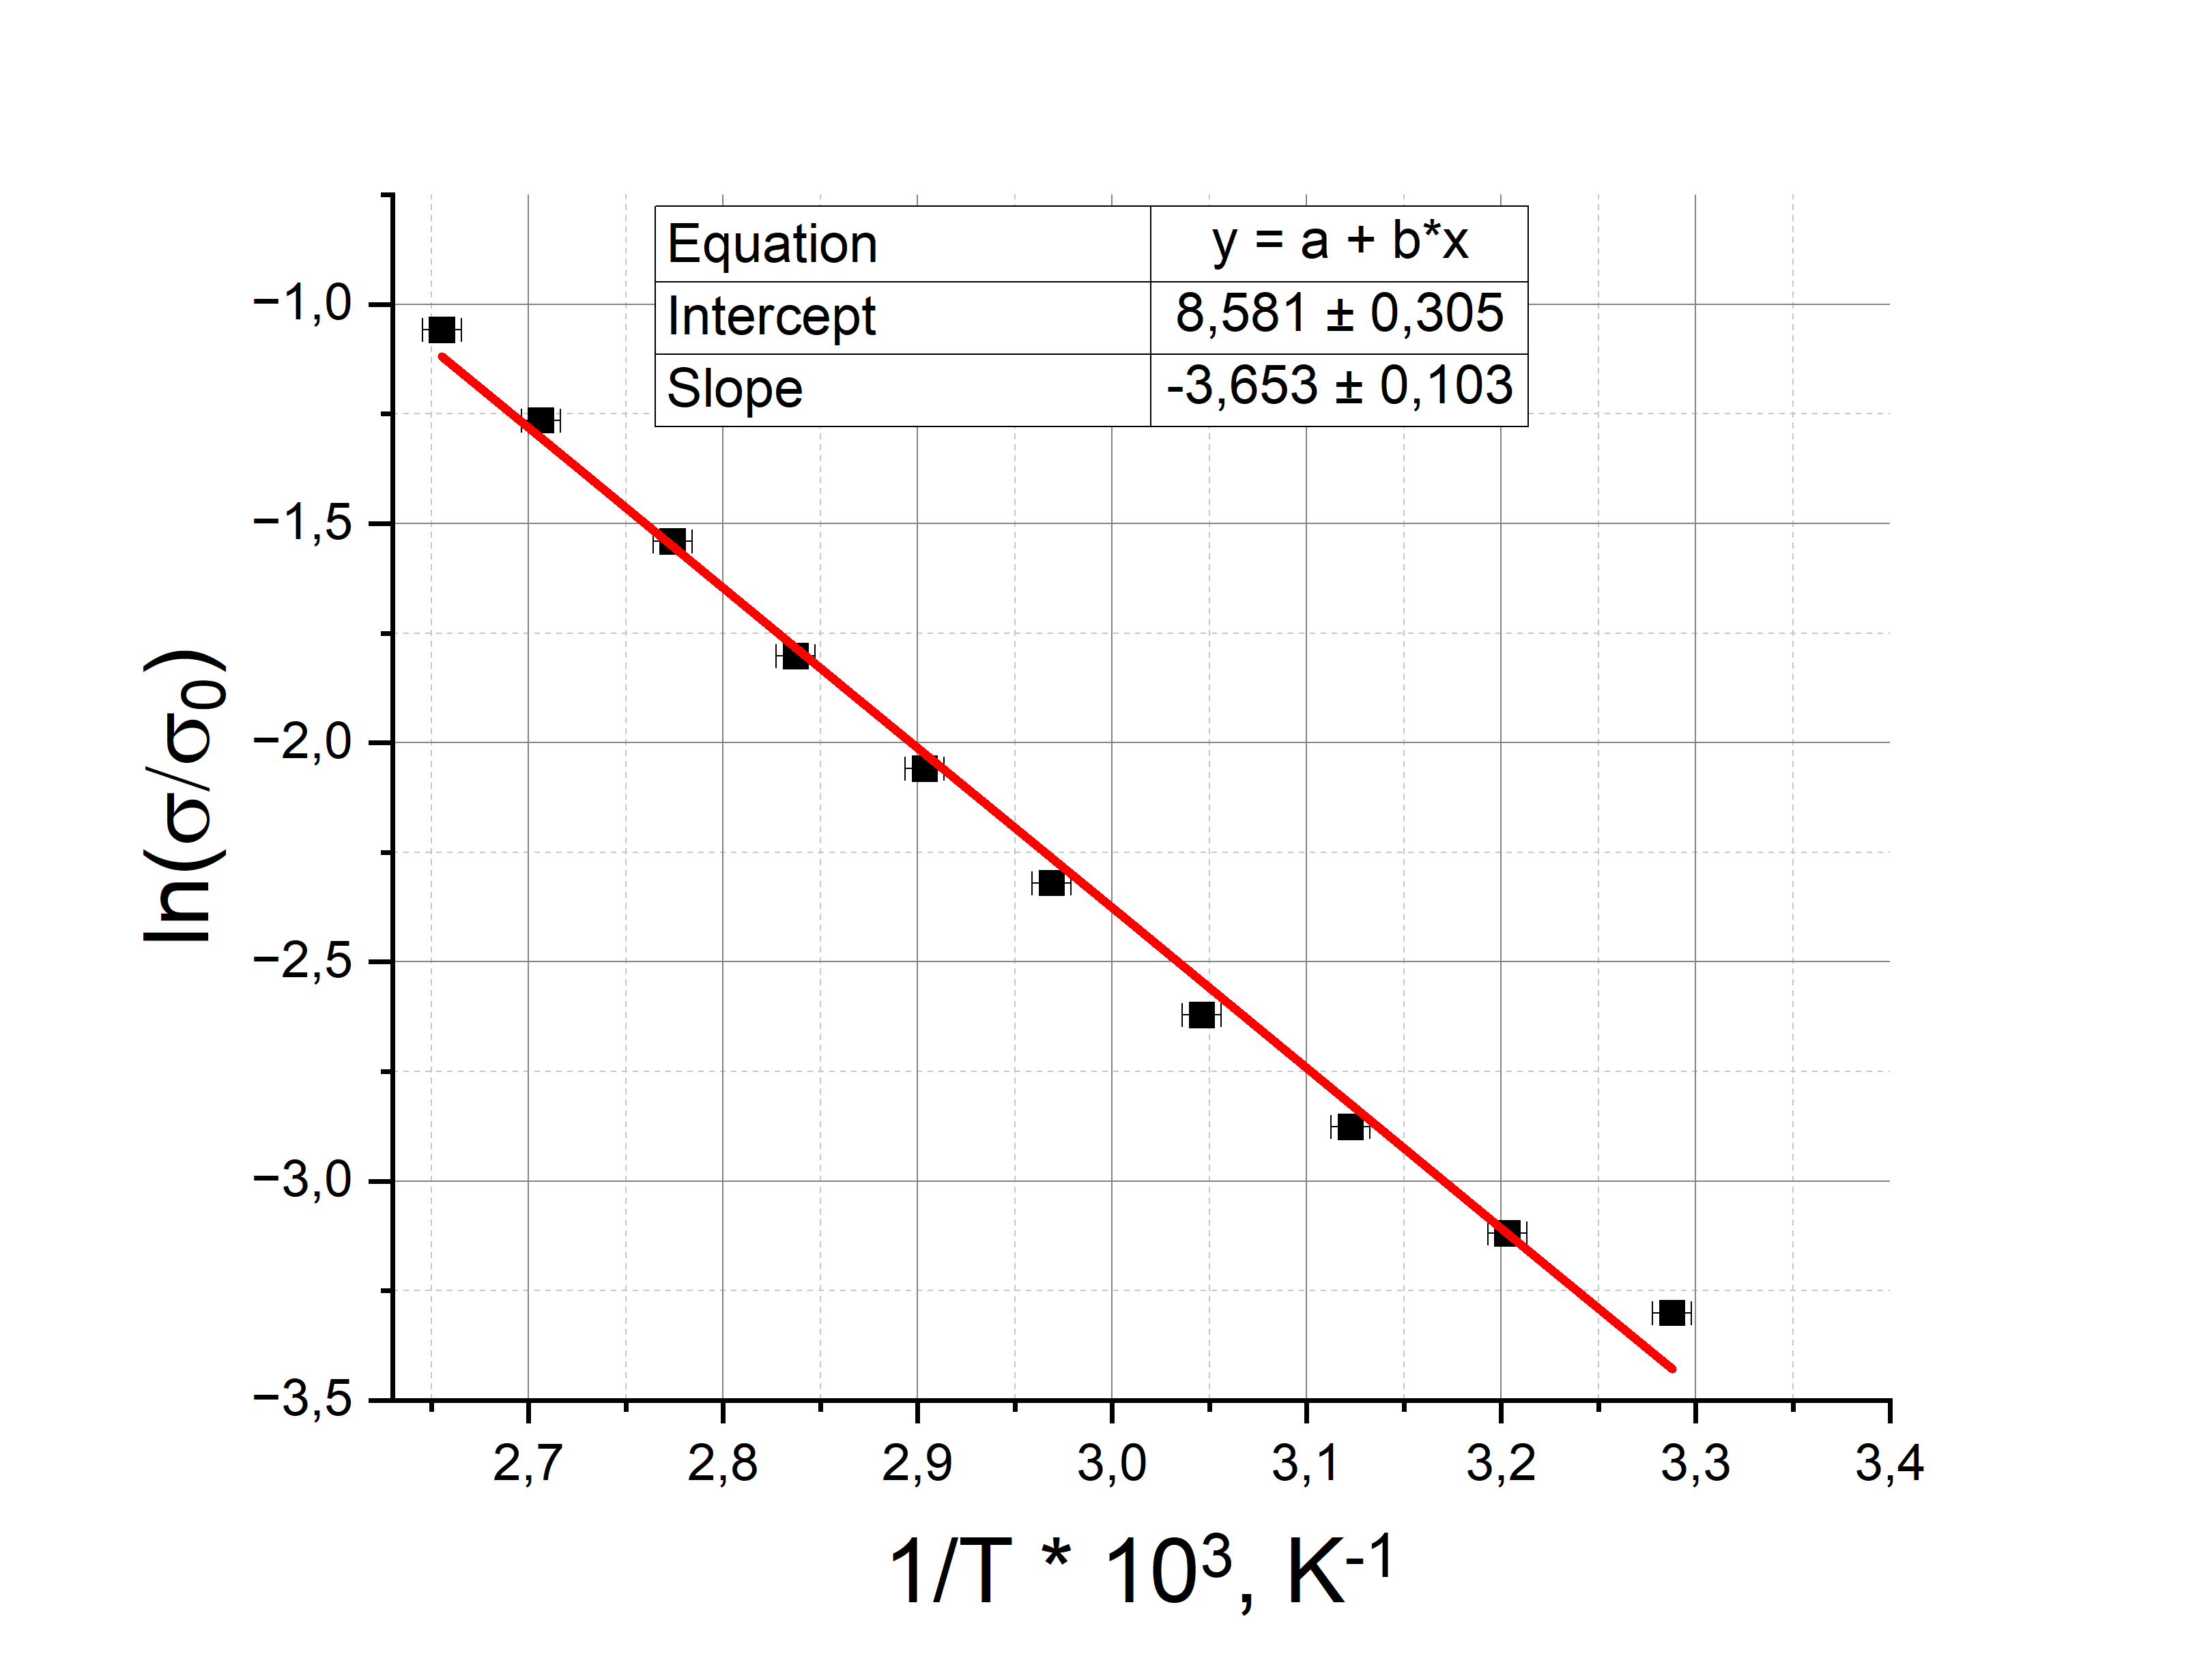
\includegraphics[width=0.8\linewidth]{linear_sigma(T)}
	\caption{Зависимость логарифма электропроводности от обратной температуры  \linebreak $\ln \left(\frac{\sigma}{\sigma_0}\right) = f \left(\frac{1}{T} \right)$}
\end{figure}

Тогда получаем значение для коэффициента наклона:

$$
	\beta = (-3,653	 \pm 0,103)\cdot 10^3 \ K
$$

Тогда из соотношения (\ref{eq5:dependence_of_temperature}) можно оценить ширину запрещенной зоны полупроводника:

\begin{align*}
	\Delta = -2k \cdot \beta \approx 0,63 \ эВ \\
	\delta_{\Delta} = -2k \cdot \delta_{\beta} \approx 0,02\ эВ 
\end{align*}

Тогда окончательно:

$$
	\Delta = (0,63 \pm 0,02) \ эВ
$$

\section*{Выводы}
\begin{itemize}
	\item В ходе работы была получена зависимость электропроводности образца полупроводника от температуры.
	\item Используя полученную зависимость, была оценена ширина запрещенной зоны образца $\Delta = (0,63 \pm 0,2) \ эВ$ 
	\item Из табличных данных, ширина запрещенной зоны для германия при комнатной температуре $\Delta = 0,67 \ эВ$. Следовательно, можно предположить, что наш образец был сделан из германия.
\end{itemize}

\section*{Приложение}

В приложении приведем график зависимости электропроводности образца от обратной температуры $\sigma = f(1/T)$

\begin{figure}[h!]
	\centering
	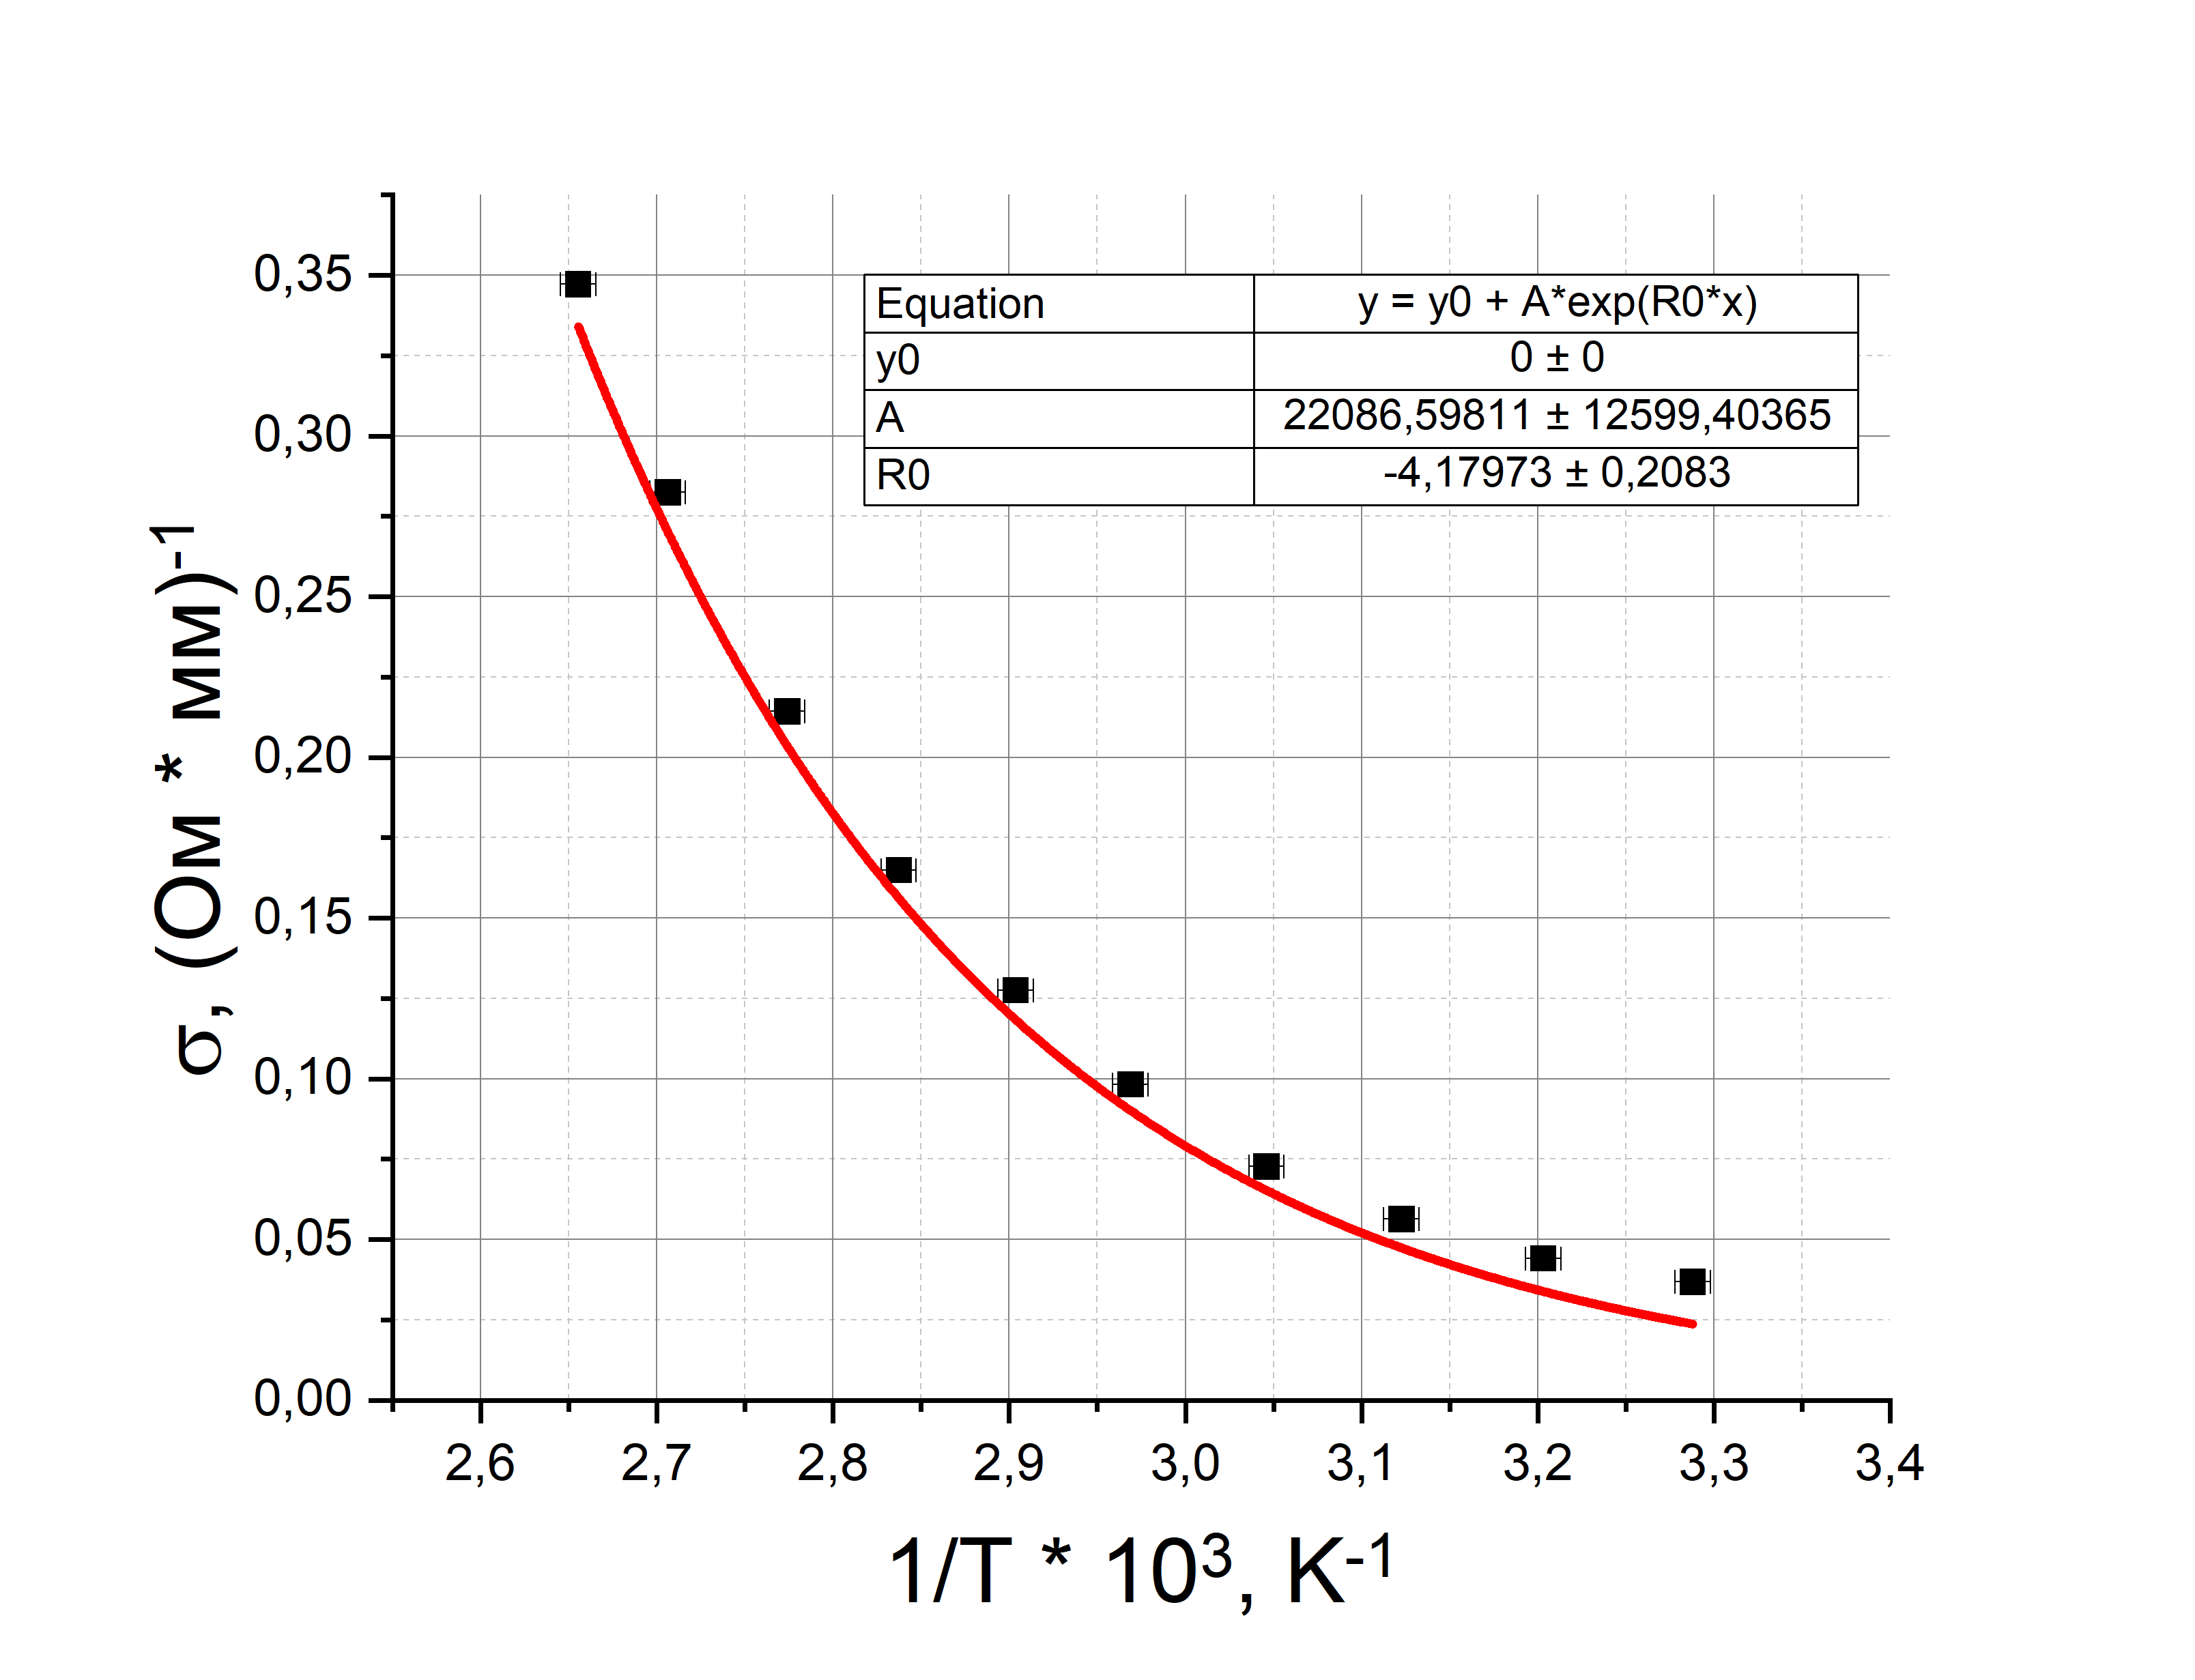
\includegraphics[width=0.7\linewidth]{exp_sigma(T)}
	\caption{Зависимость электропроводности от обратной температуры $\sigma = f(1/T)$}
\end{figure}

\begin{thebibliography}{2}
\bibitem{goldin}
Гольдин Л.Л., Новикова Г.И. Квантовая физика. Вводных курс. 2016.
\bibitem{lab}
Игошин Ф. Ф., Самарский Ю. А., Ципенюк Ю. М. Лабораторный практикум по общей физике: квантовая физика. 2012.
\end{thebibliography}


\end{document}

